\chapter{Геймификация бега}
Для геймификации бега была придумана концепция интерактивного сюжета, в рамках которой игрок оказывается в некой ситуации, разворачивающейся по мере прохождения точек интереса на карте. Также по мере развития сюжета игроку предлагаются некоторые препятствия, которые он должен физически обойти.
\section{Интерактивный сценарий}
Интерактивный сценарий представляет из себя иерархическую структуру данных cо вложенными объектами разного типа.
Техническая реализация сценария представляет из себя JSON-файл с жёстко заданной структурой. Основные компоненты сценария приведены на рис. \ref{fig:scenario_components}.

На схеме представлены следующие объекты:
\begin{description}
	\item[Chapter] Глава. Представляет из себя единицу геймифицированной тренировки, содержит собственный набор игровых объектов, актуальных для конкретной игровой сессии, как-то: Игровые события и Точки интереса на карте.
	\item[Event] Игровое событие. Игровые события описаны подробнее в разделе \ref{sec:events}.
	\item[Geofencing] Точки интереса на карте. Информация о точках интереса на карте представлена в разделе \ref{sec:geofencing}.
\end{description}

\begin{figure}[H]
	\centering
	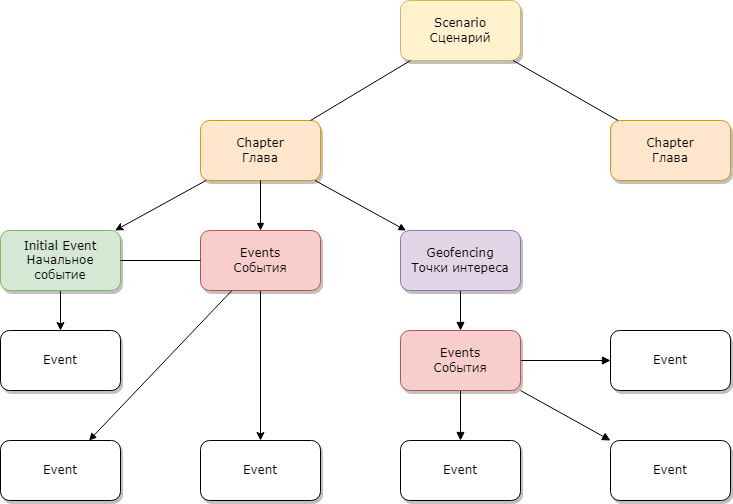
\includegraphics[width=\textwidth]{flesh/runGamification/scenario.png}
	\caption{\label{fig:scenario_components}Схема компонентов сценария}
\end{figure}

\section{Действия, производимые игрой}
\label{sec:actions}
Во время активной сессии игра может вызывать различные действия, основываясь на их контексте. Под контекстом будем понимать один из трёх над-родительских для действия объектов:
\begin{itemize}
	\item Начальное событие главы.
	\item Промежуточное событие главы.
	\item Событие для точки интереса на карте.
\end{itemize}
У каждого действия есть свой набор атрибутов, при этом у каждого действия обязательно есть следующие методы:
\begin{description}
	\item[initTimer] Данный метод возвращает инициализированный объект типа CountDownTimer, представляющий из себя таймер обратного отсчёта, по истечении которого будет запущен код, начинающий выполнение игрового действия. Такая реализация позволяет планировать действия на будущее в рамках активной игровой сессии.
	\item[finishTimer] Данный метод может не требоваться для действия, поэтому он возвращает  nullable объект типа CountDownTimer?, представляющий из себя таймер обратного отсчёта, по истечении которого будет запущен код, завершающий выполнение игрового действия. Такая реализация позволяет финализировать запущенные действия и валидировать результат их выполнения, если это необходимо.
\end{description}
\smallskip
Актуальная версия приложения имеет возможность вызывать два типа игровых действий:
\begin{itemize}
	\item Воспроизведение аудиоконтента.
	\item Генерация виртуального препятствия.
\end{itemize}
\smallskip
Далее рассмотрим их подробнее.

\subsection*{Действие воспроизведения аудиоконтента}
Данное действие воспроизводит заданный в файле сценария аудиотрек из вложенных в приложение ресурсов.

Этот вид действия не требует таймер финализации, т.к. для запуска трека достаточно только таймера запуска, и после его выполнения не требуется проводить проверки.

\subsection*{Действие генерации виртуального препятствия}
Данное действие генерирует заданное в файле сценария препятствие из реализованных в приложении. Детальная информация о виртуальных препятствиях представлена в разделе \ref{sec:obstacles}.

Это действие обязательно имеет оба таймера, так как у препятствия есть метод запуска и метод финализации, проверяющий было ли препятствие преодолено.
 
\section{Система игровых событий}
\label{sec:events}
Игровое событие представляет из себя набор игровых действий с соответствующими их типам атрибутами, которые игра может вызвать в некоторый момент времени на протяжении игровой сессии.

В приложении предусмотрено три типа игровых событий:
\begin{description}
	\item [Начальное событие] Если задано, вызывается всегда в начале соответствующей главы сценария
	\item [Событие, привязанное ко времени] Обязательно имеет атрибут с задержкой в секундах от начала главы, и вызывается в соответствующий момент времени.
	\item [Событие, не привязанное ко времени] Как и предыдущий тип, данное событие вызывается в определённый момент времени, но, в отличие от предыдущего, задержка не задаётся в сценарии, а рассчитывается в момент генерации как псевдослучайное число между двумя границами из кода приложения.
\end{description}


\section{Система виртуальных препятствий}
\label{sec:obstacles}
Виртуальное препятствие является концептом, которого не существует в реальном мире, но он генерируется игрой и заставляет игрока выполнить какое-либо действие, связанное с бегом. Сейчас мы различаем следующие виды препятствий:
\begin{description}
	\item[Дикие собаки] Данное препятствие имитирует бег за игроком диких собак, которые могут нанести ему вред : для преодоления препятствия необходимо ускориться за определённое время.
	\item[Сильный ветер] Данное препятствие имитирует сильный ветер, сносящий игрока. Для преодоления препятствия необходимо ``подыграть'' игре и снизить скорость за определённое время.
\end{description}
\smallskip
Данные препятствия выбраны исходя из концепции интервальных тренировок и режима бега, при котором человеку необходимо чередовать ускорение и замедление в рамках одной игровой сессии.

У каждого препятствия есть атрибут статуса, принимающий одно из следующих значений:
\begin{description}
	\item[UNKNOWN] Неизвестный статус. Присваевается препятствию в случае непредвиденных технических ошибок. При штатной работе приложения препятствия с таким статусом отсутствуют.
	\item[ONGOING] Активное препятствие. Приложение ожидает завршения таймера для валидации состояния преодоления.
	\item[FAILED] Завршенное непреодолённое препятствие. По завершении таймера приложение определило, что игрок не преодолел препятствие.
	\item[SUCCEEDED] Завршенное преодолённое препятствие. По завершении таймера приложение определило, что игрок смог преодолеть препятствие.
\end{description}
\smallskip
Далее рассмотрим некоторые детали работы с виртуальными препятствиями.
\subsection*{Генерация препятствия}
При генерации препятствия происходят следующие действия:
\begin{enumerate}
	\item Сохранение препятствия как активного в менеджере препятствий.
	\item Сохранение препятствия в репозиторий сгенерированных препятствий.
	\item Вызов инициализирующего метода препятствия.
	\item Запуск голосовой инструкции о типе препятствия и способе его преодоления.
\end{enumerate}

\subsection*{Валидация препятствия}
После срабатывания таймера финализации действия, отвечающего за финализацию препятствия вызывается соответствующий метод активного препятствия из менеджера препятствий и происходит следующее:
\begin{enumerate}
	\item Определение статуса преодоления препятствия.
	\item Обновление сущности в репозитории.
	\item Запуск голосовой инструкции о результате преодоления препятствия.
\end{enumerate}

\section{Система точек интереса}
\label{sec:geofencing}
Для геймификации и имитации продвижения по сюжетной линии сценария была реализована возможность менять игровой контекст по достижении очередной точки интереса на карте.

Точка интереса на карте представляет из себя объект с географическими координатами, рядом дополнительных атрибутов и набором игровых событий, каждое со своими атрибутами. При нахождении устройства пользователя в некоторой окрестности актуальной на момент игровой сессии точки игра может вызвать событие из набора событий данной точки.

Обработка точек интереса на карте производится методами Geofencing (см. разделы \ref{subsec:geodata} и \ref{subsubsec:geofencing_manager}).

Игровые события, вызываемые на входе пользователя в отслеживаемую зону, технически и идейно соответствуют уже рассмотренным в разделе \ref{sec:events}.

Отслеживание входа устройства игрока в заданную зону производится в рамках следующих ограничений:
\begin{itemize}
	\item Отслеживание ведётся только во время активной игровой сессии.
	\item Отслеживается нахождение пользователя только относительно одной актуальной в данный момент времени точки интереса (а таковая может быть только одна).
	\item Отслеживается только вход в заданную радиусом область. Технически есть возможность также отслеживать длительное нахождение в ней и выход из этой области, но в рамках данной работы эти события не отслеживаются.
\end{itemize}